%\documentclass[11pt]{beamer}
\documentclass[11pt,pdf]{beamer}
\mode<presentation>{}
\usetheme{Warsaw}
\usecolortheme{whale}
\setbeamercolor{structure}{fg=blue!55!black}
\usepackage[utf8]{inputenc}
\usepackage{amsmath}
\usepackage{amsfonts}
\usepackage{amssymb}
\addtobeamertemplate{navigation symbols}{}{%
	\usebeamerfont{footline}%
	\usebeamercolor[fg]{footline}%
	\hspace{1em}%
	\insertframenumber/\inserttotalframenumber
}
\setbeamercolor{footline}{fg=black!20!blue}
\setbeamerfont{footline}{series=\bfseries}
\setbeamertemplate{caption}[numbered]
\usepackage{graphicx}
\usepackage{color}
\useoutertheme{split}
\renewcommand{\baselinestretch}{1.2}

\begin{document}
%	\author{Mr Olumide \& Mrs Anuoluwapo Oyalola}
	\title{Mr Olumide \& Mrs Anuoluwapo Oyalola \\ Child Naming Ceremony}
	%\subtitle{}
	%\logo{}
	\institute{\textbf{Anchored by: Pastor Babalola}}
	\date{\small{Date: Saturday, 7th October 2017 \\ Time: 12 Noon}}
	%\subject{}
	%\setbeamercovered{transparent}
	%\setbeamertemplate{navigation symbols}{}
	\begin{frame}
	\transblindsvertical
	\titlepage
\end{frame}
\section{Now the Child Names}

\begin{frame}{Baby}
\textcolor{blue!45!black}{\Large{Immediately after birth}}
\begin{figure}[t]
	\centering
	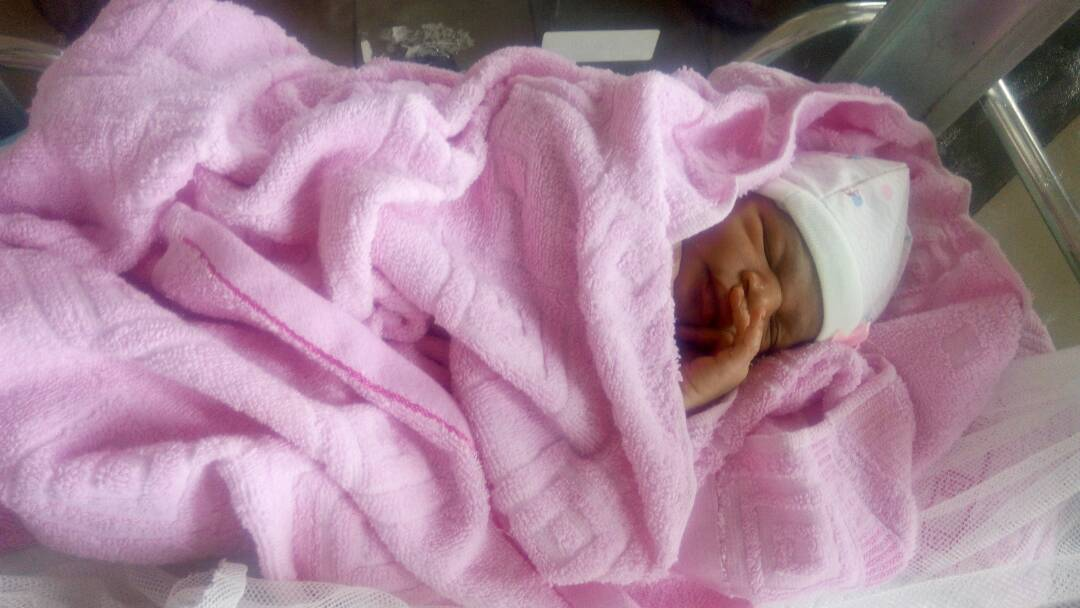
\includegraphics[width=1.01\linewidth]{Images/Morireoluwa1.jpeg}
	%\caption[R GUI]{}
	%\caption{$\mathrm{\huge{R}}$ GUI}
	%\label{fig:RPage}
\end{figure}
\end{frame}


\begin{frame}{Baby}
\begin{figure}[t]
	\centering
	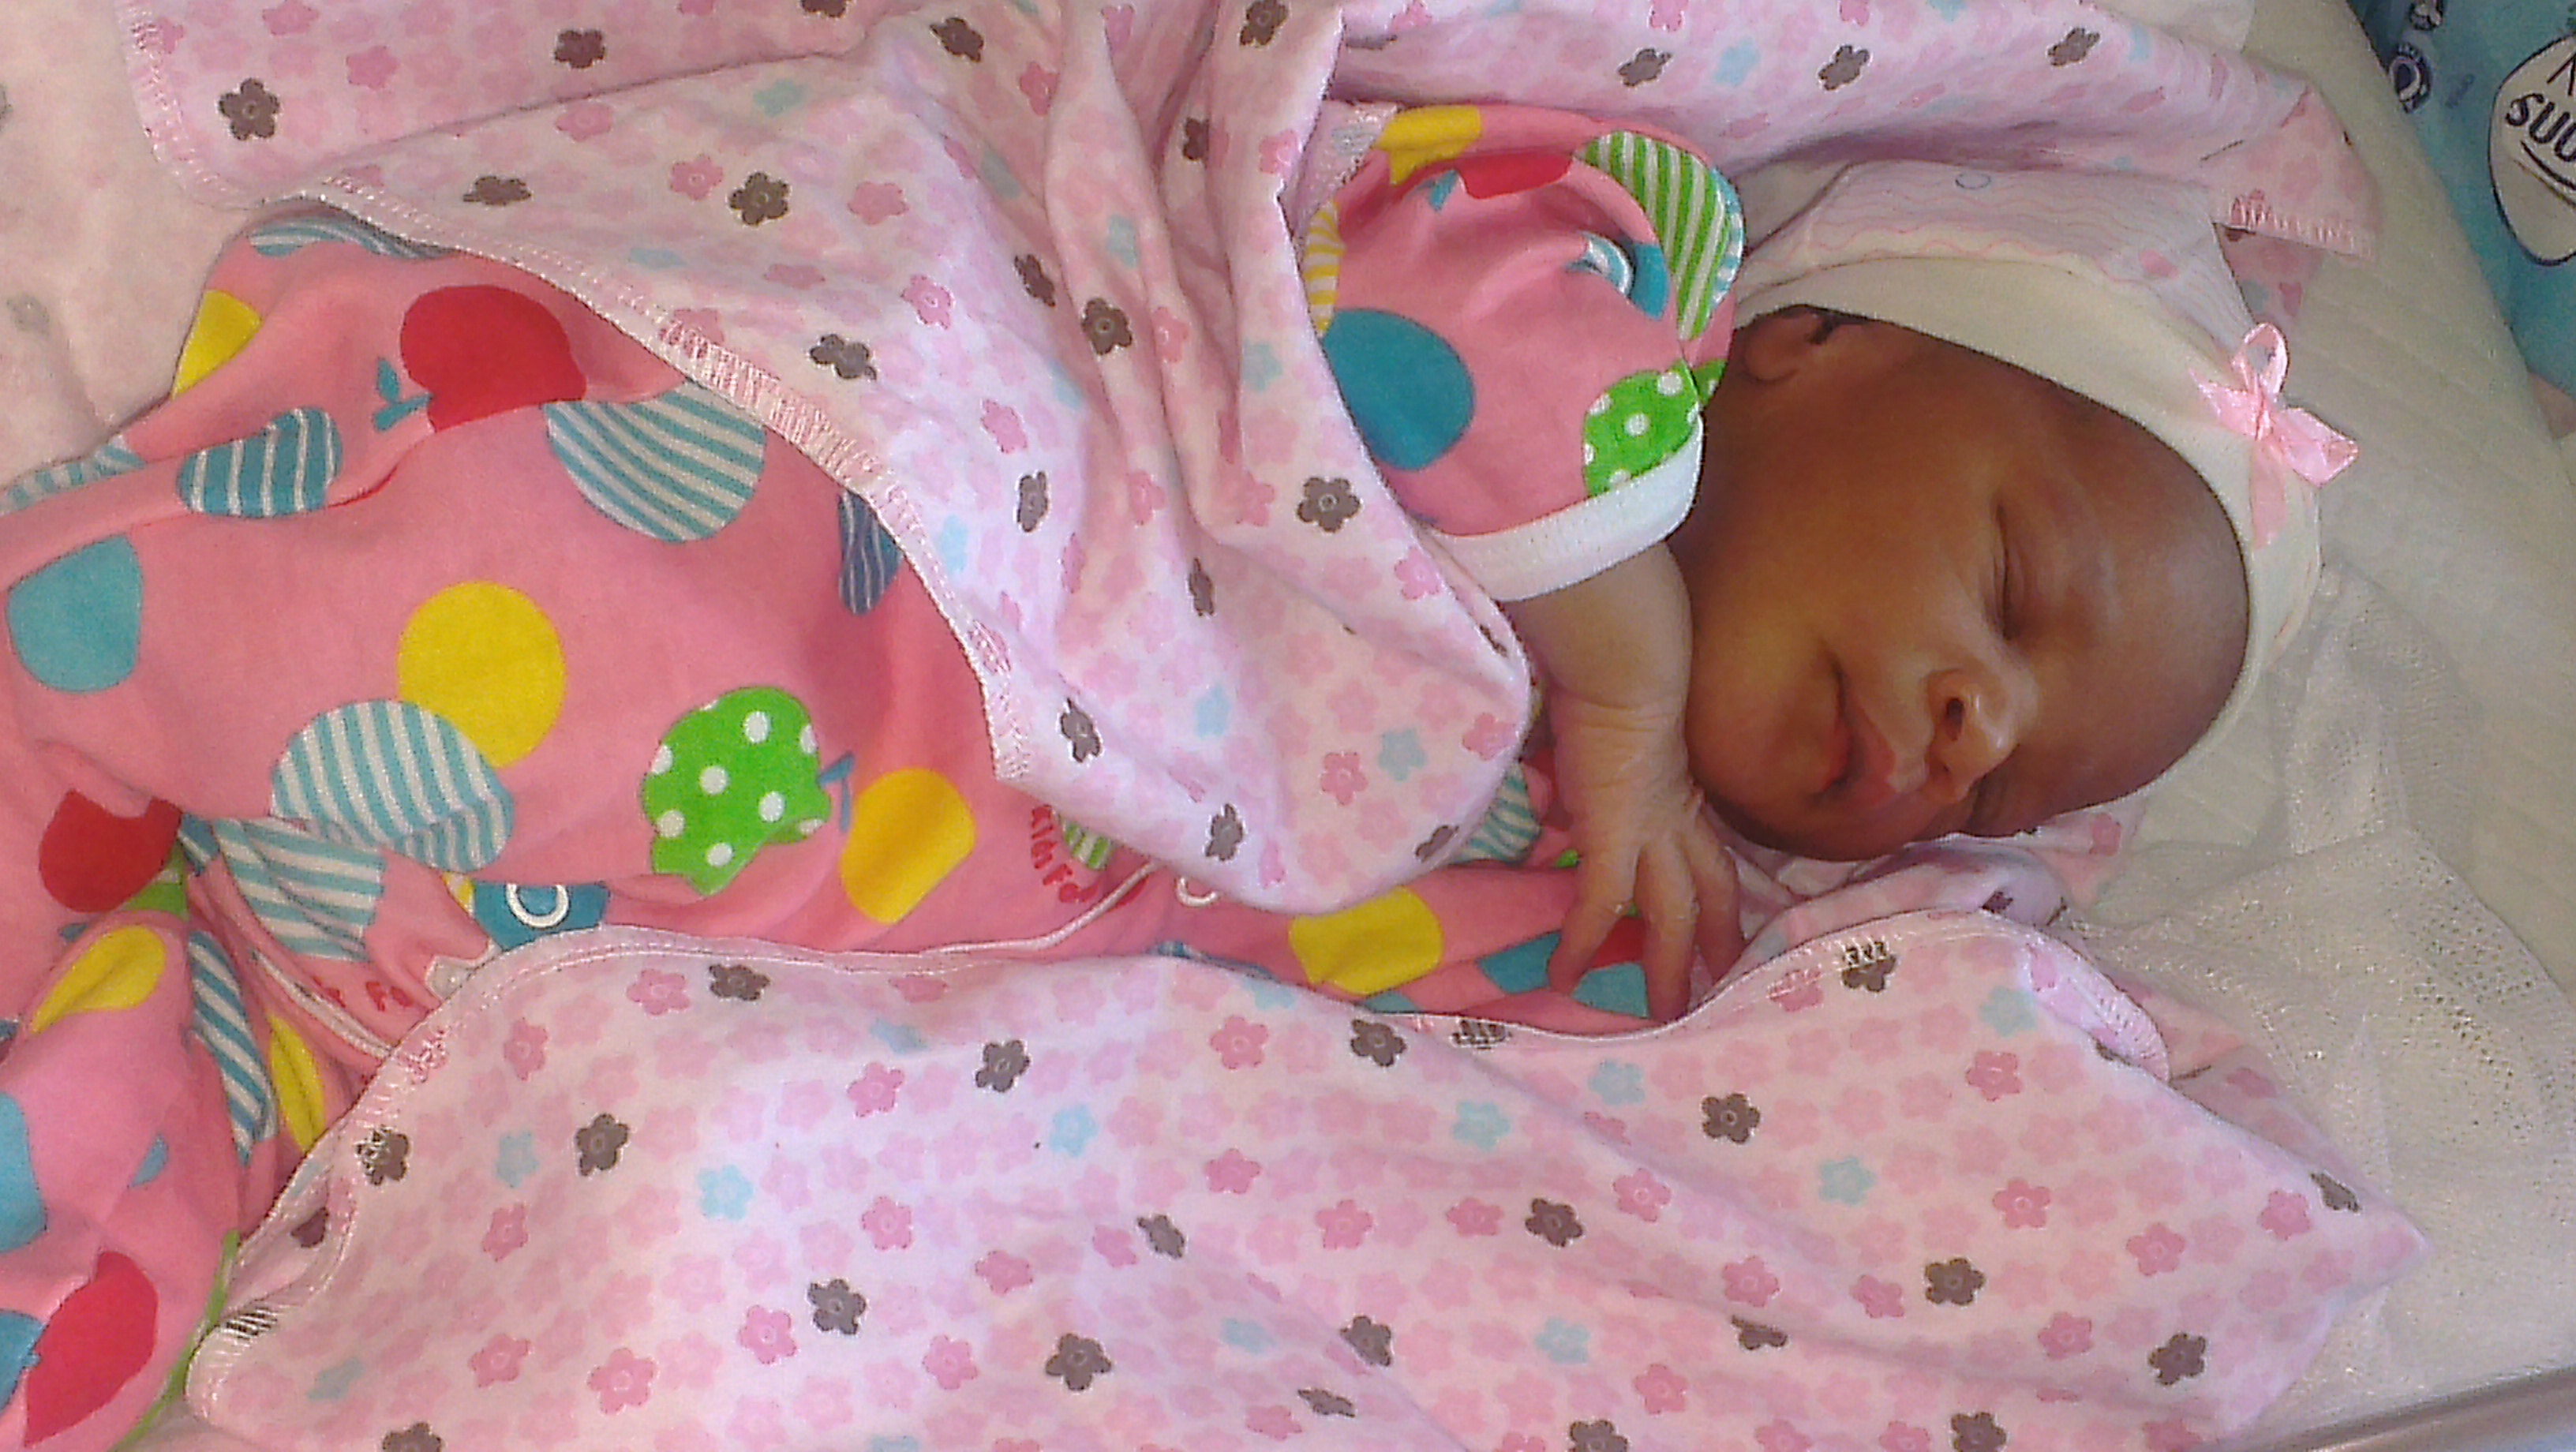
\includegraphics[width=1.01\linewidth]{Images/baby.jpg}
	%\caption[R GUI]{}
	%\caption{$\mathrm{\huge{R}}$ GUI}
	%\label{fig:RPage}
\end{figure}
\end{frame}


\begin{frame}{Baby}
\begin{figure}[t]
	\centering
	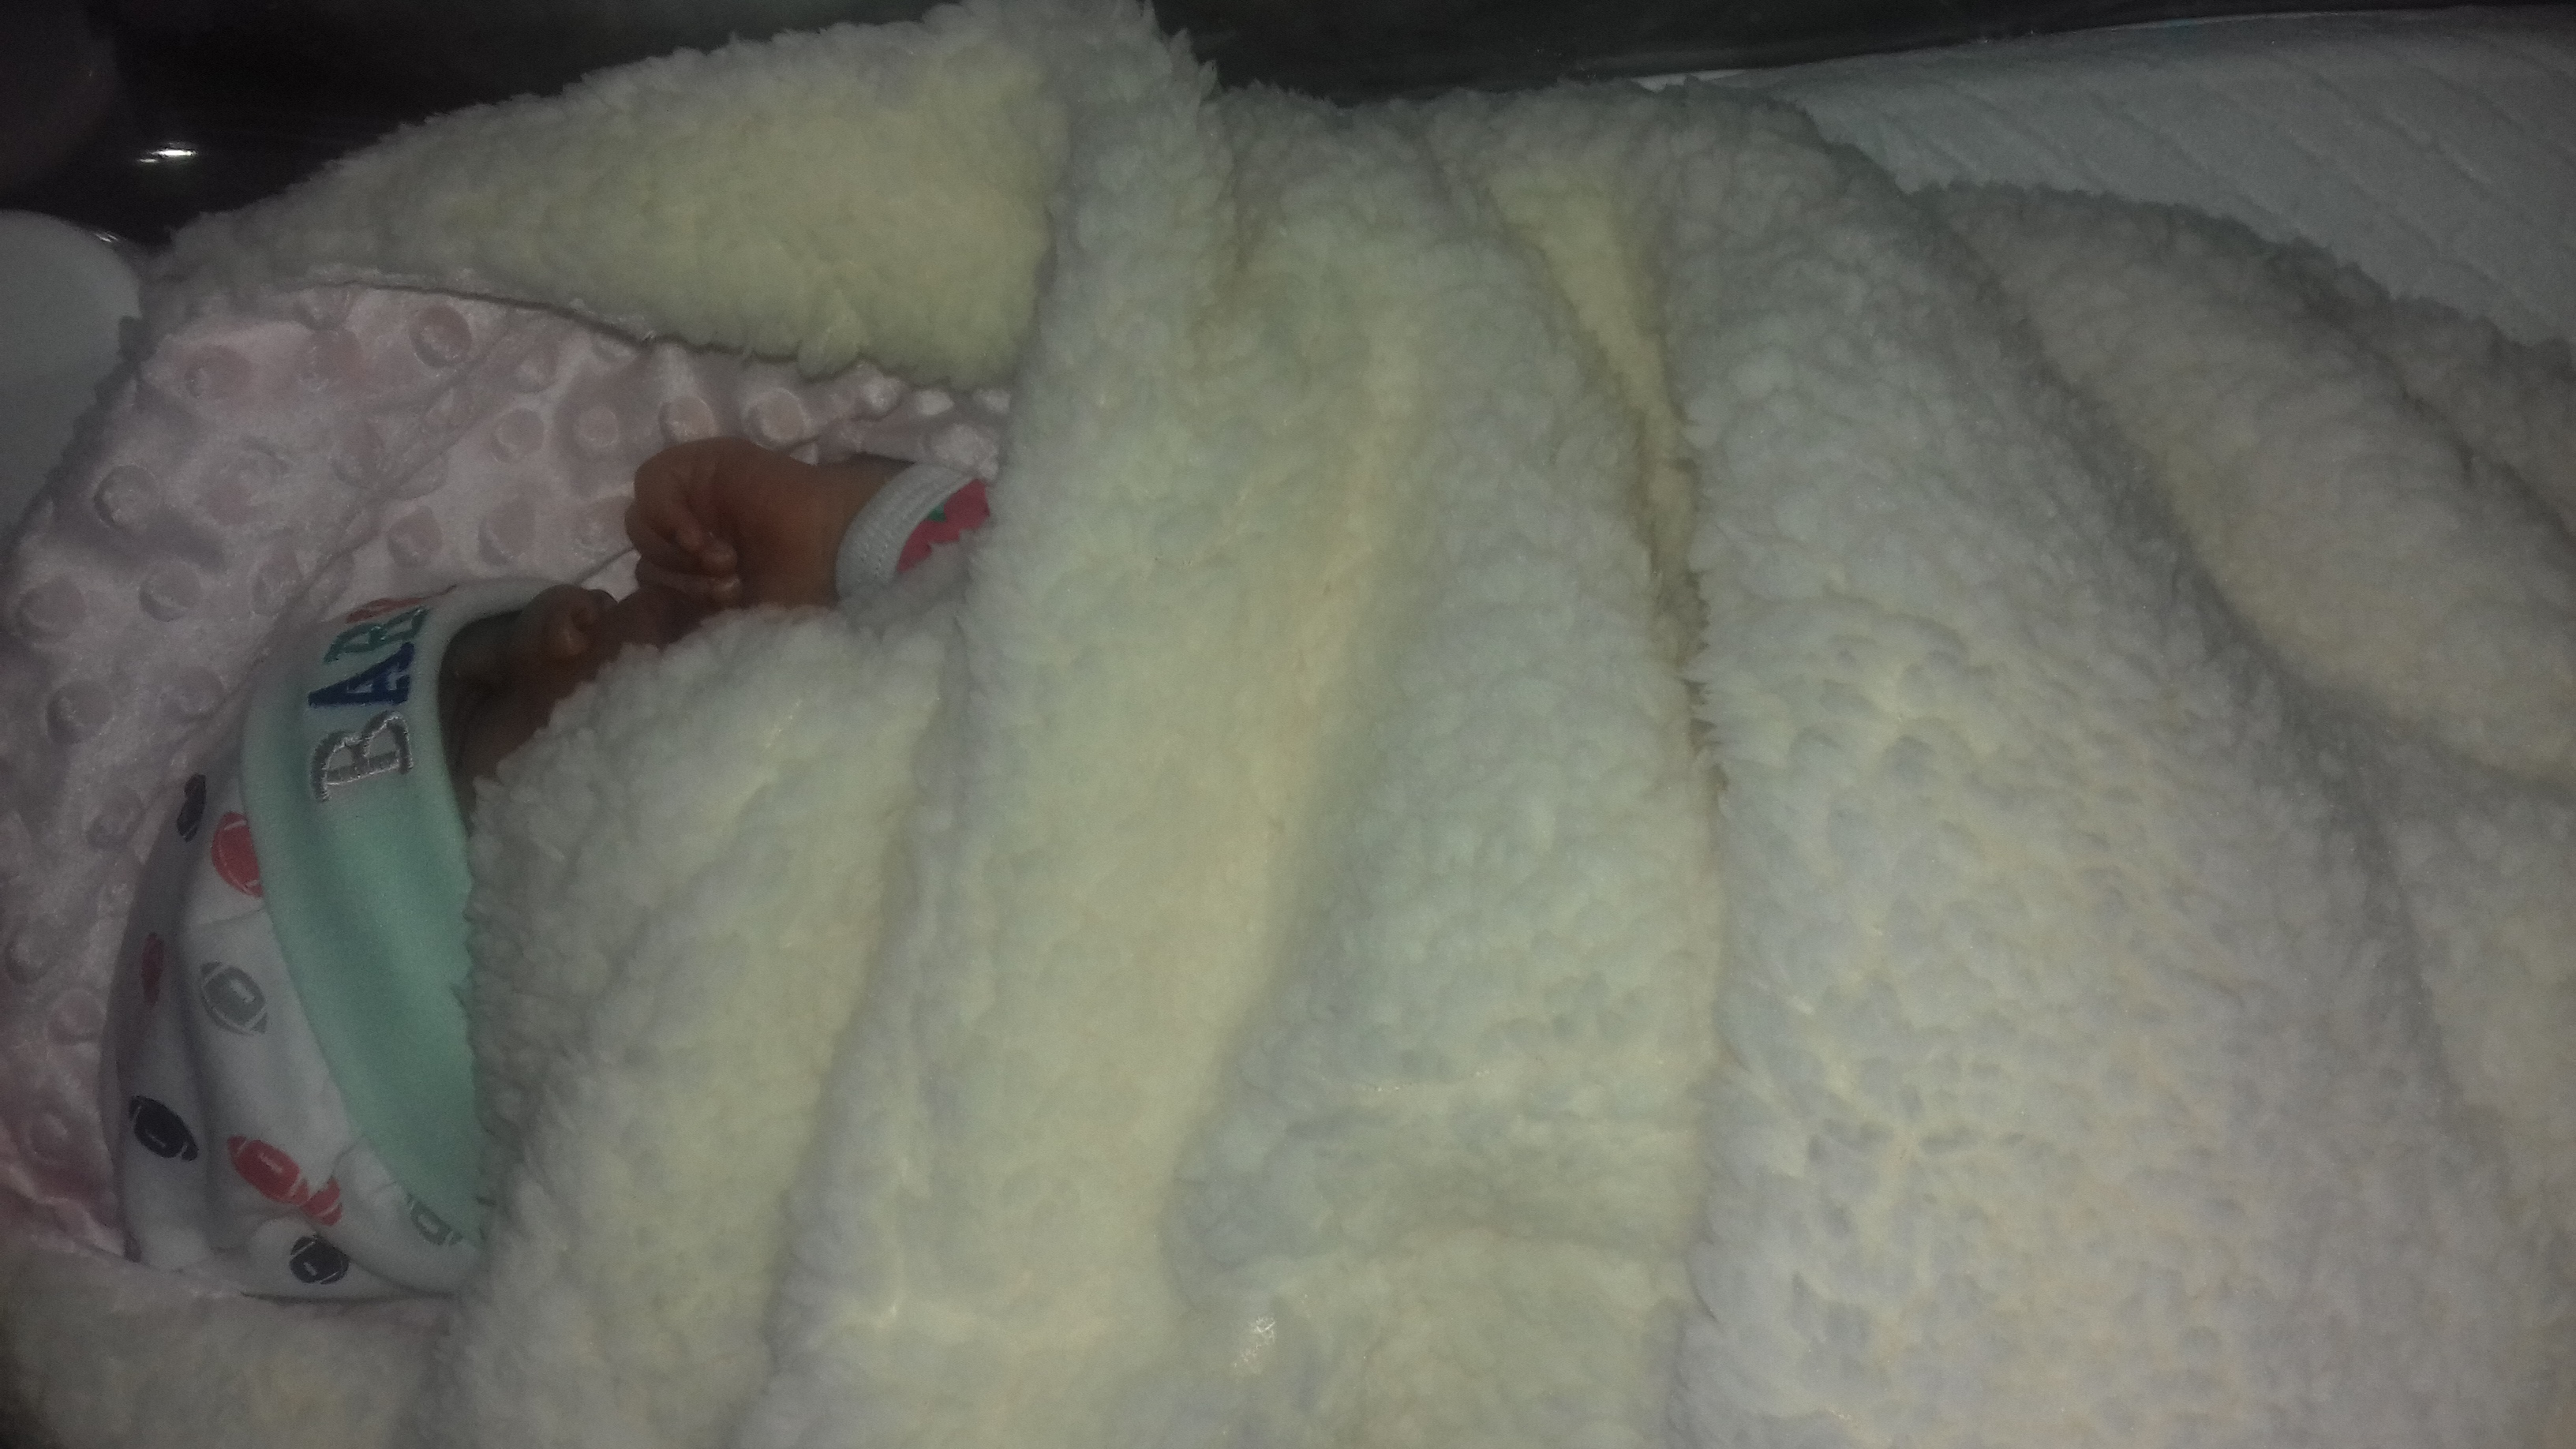
\includegraphics[width=1.03\linewidth]{Images/baby1.jpg}
	%\caption[R GUI]{}
	%\caption{$\mathrm{\huge{R}}$ GUI}
	%\label{fig:RPage}
\end{figure}
\end{frame}


\begin{frame}{Baby}
\begin{figure}[t]
	\centering
	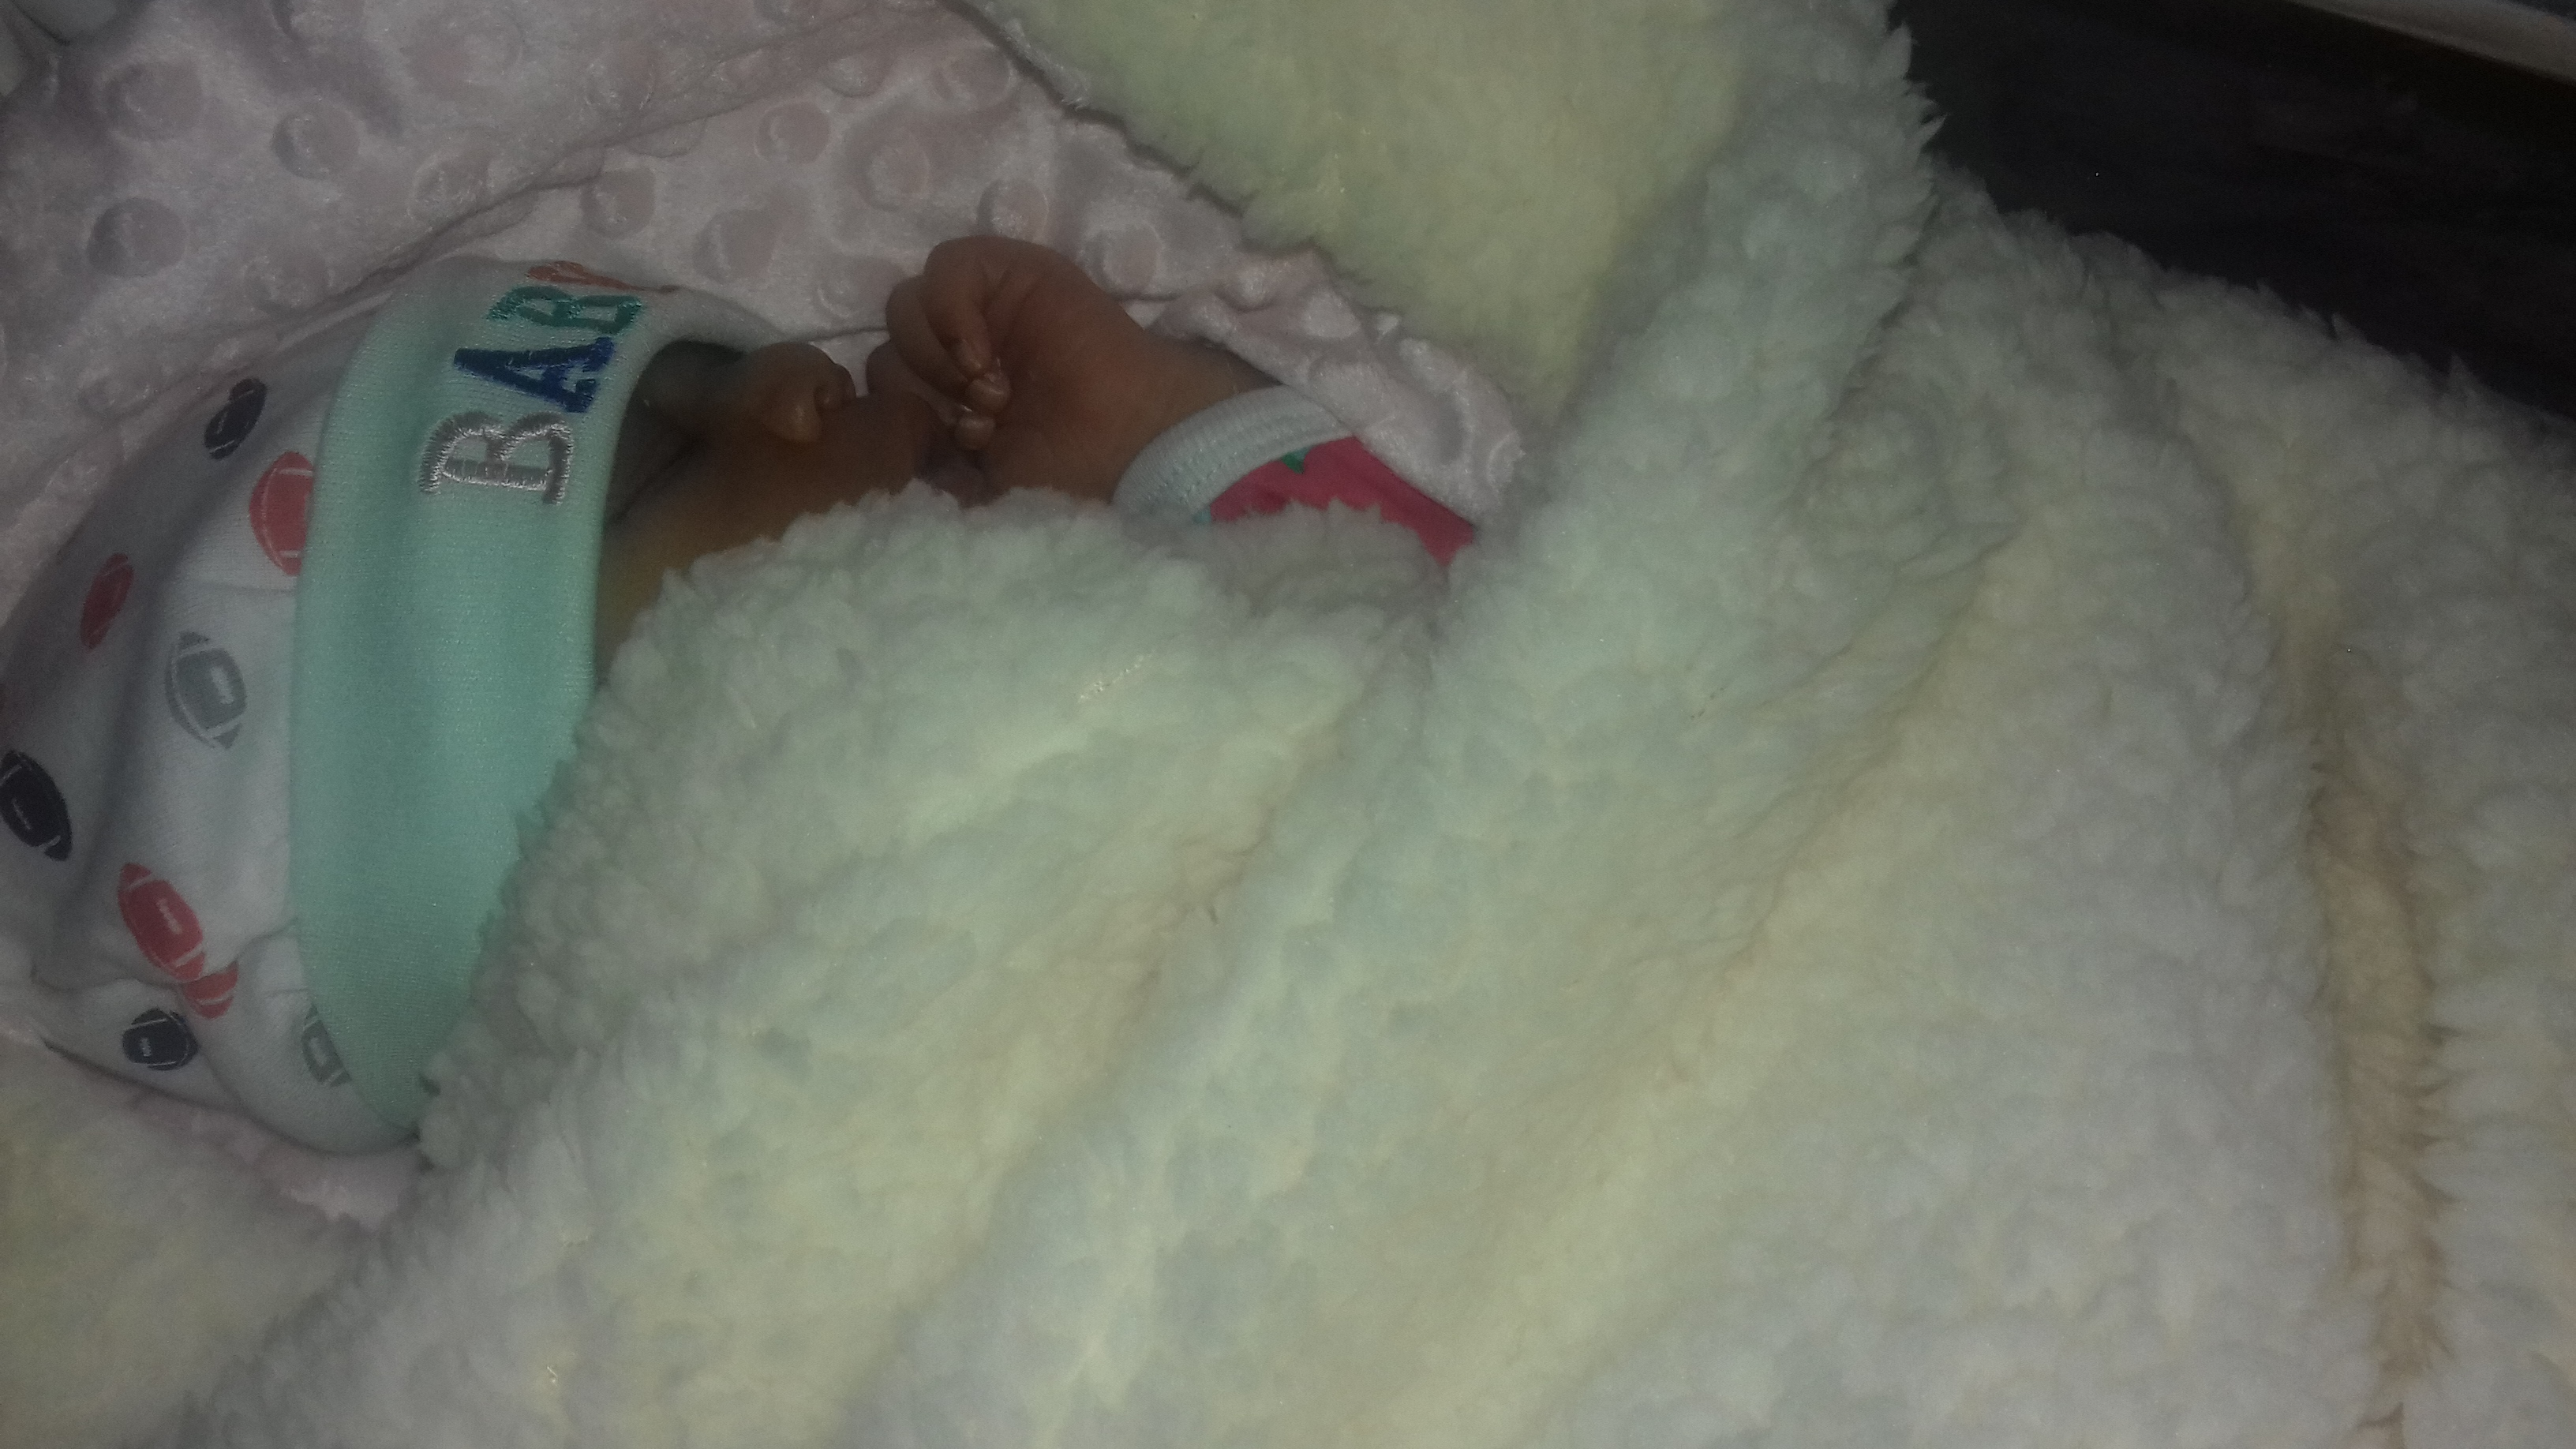
\includegraphics[width=1.03\linewidth]{Images/baby2.jpg}
	%\caption[R GUI]{}
	%\caption{$\mathrm{\huge{R}}$ GUI}
	%\label{fig:RPage}
\end{figure}
\end{frame}

\begin{frame}{Baby}
\begin{figure}[t]
	\centering
	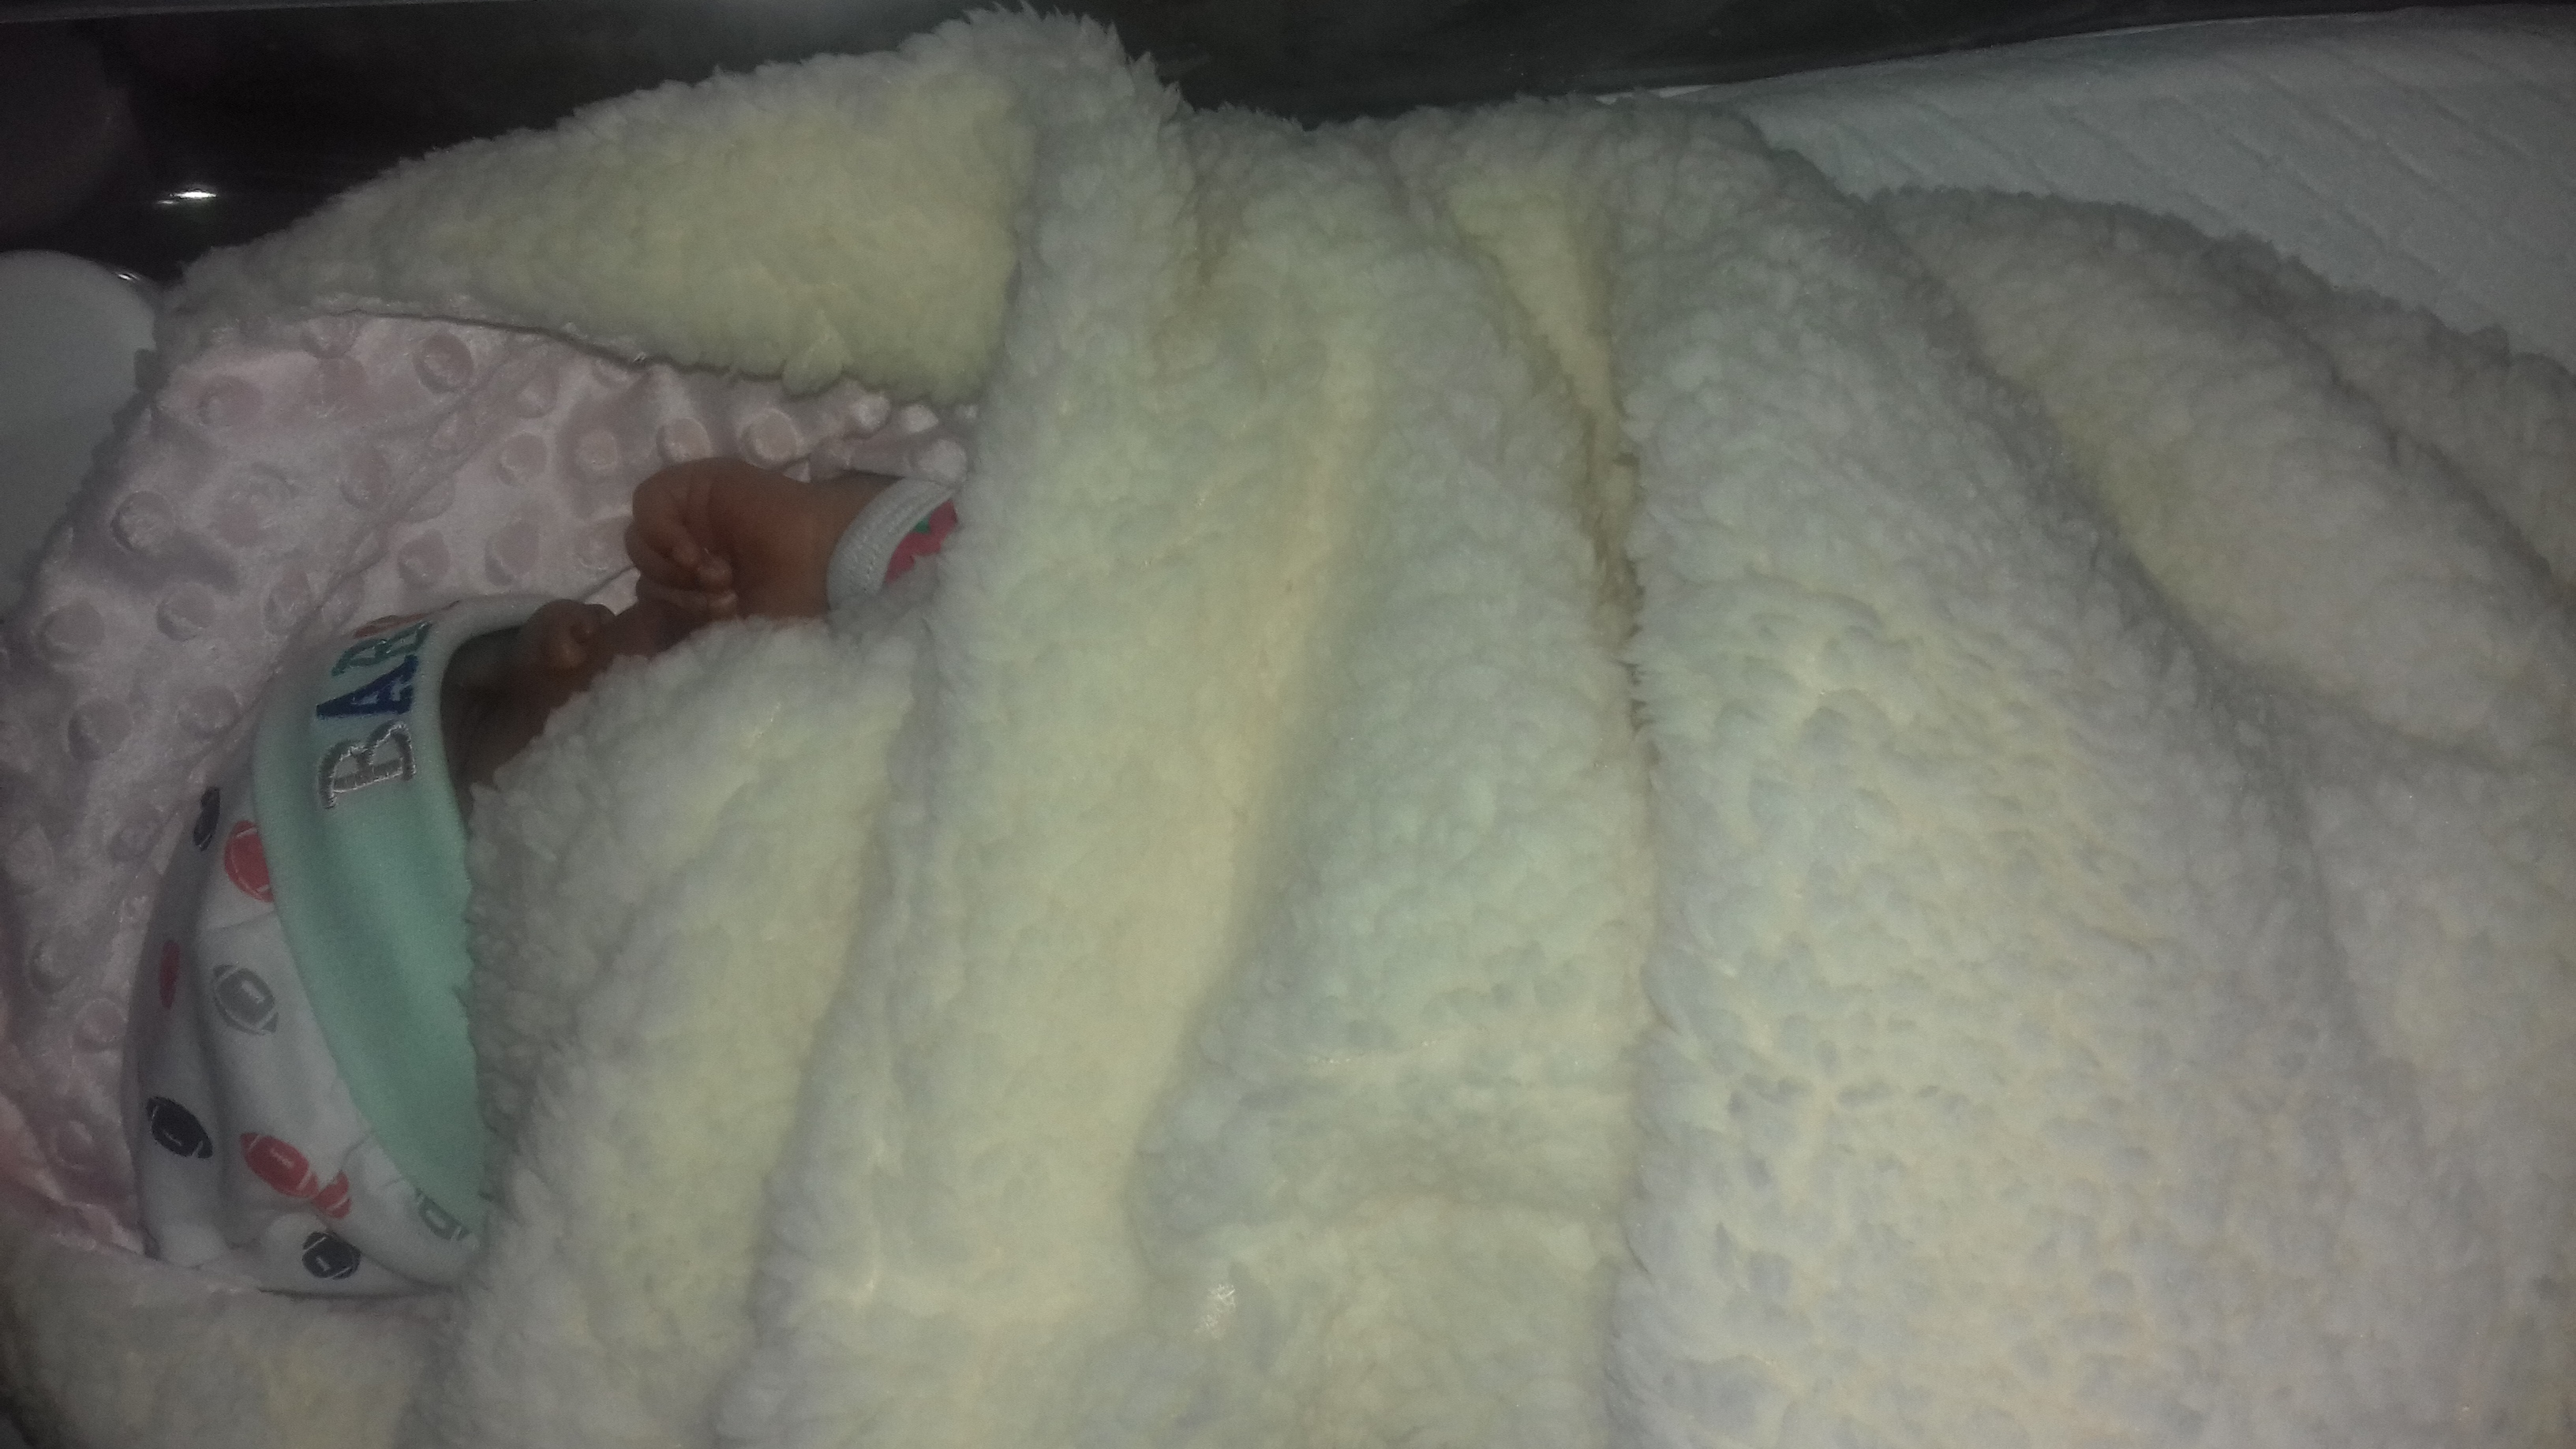
\includegraphics[width=1.03\linewidth]{Images/baby3.jpg}
	%\caption[R GUI]{}
	%\caption{$\mathrm{\huge{R}}$ GUI}
	%\label{fig:RPage}
\end{figure}
\end{frame}

\begin{frame}{Baby}
\begin{figure}[t]
	\centering
	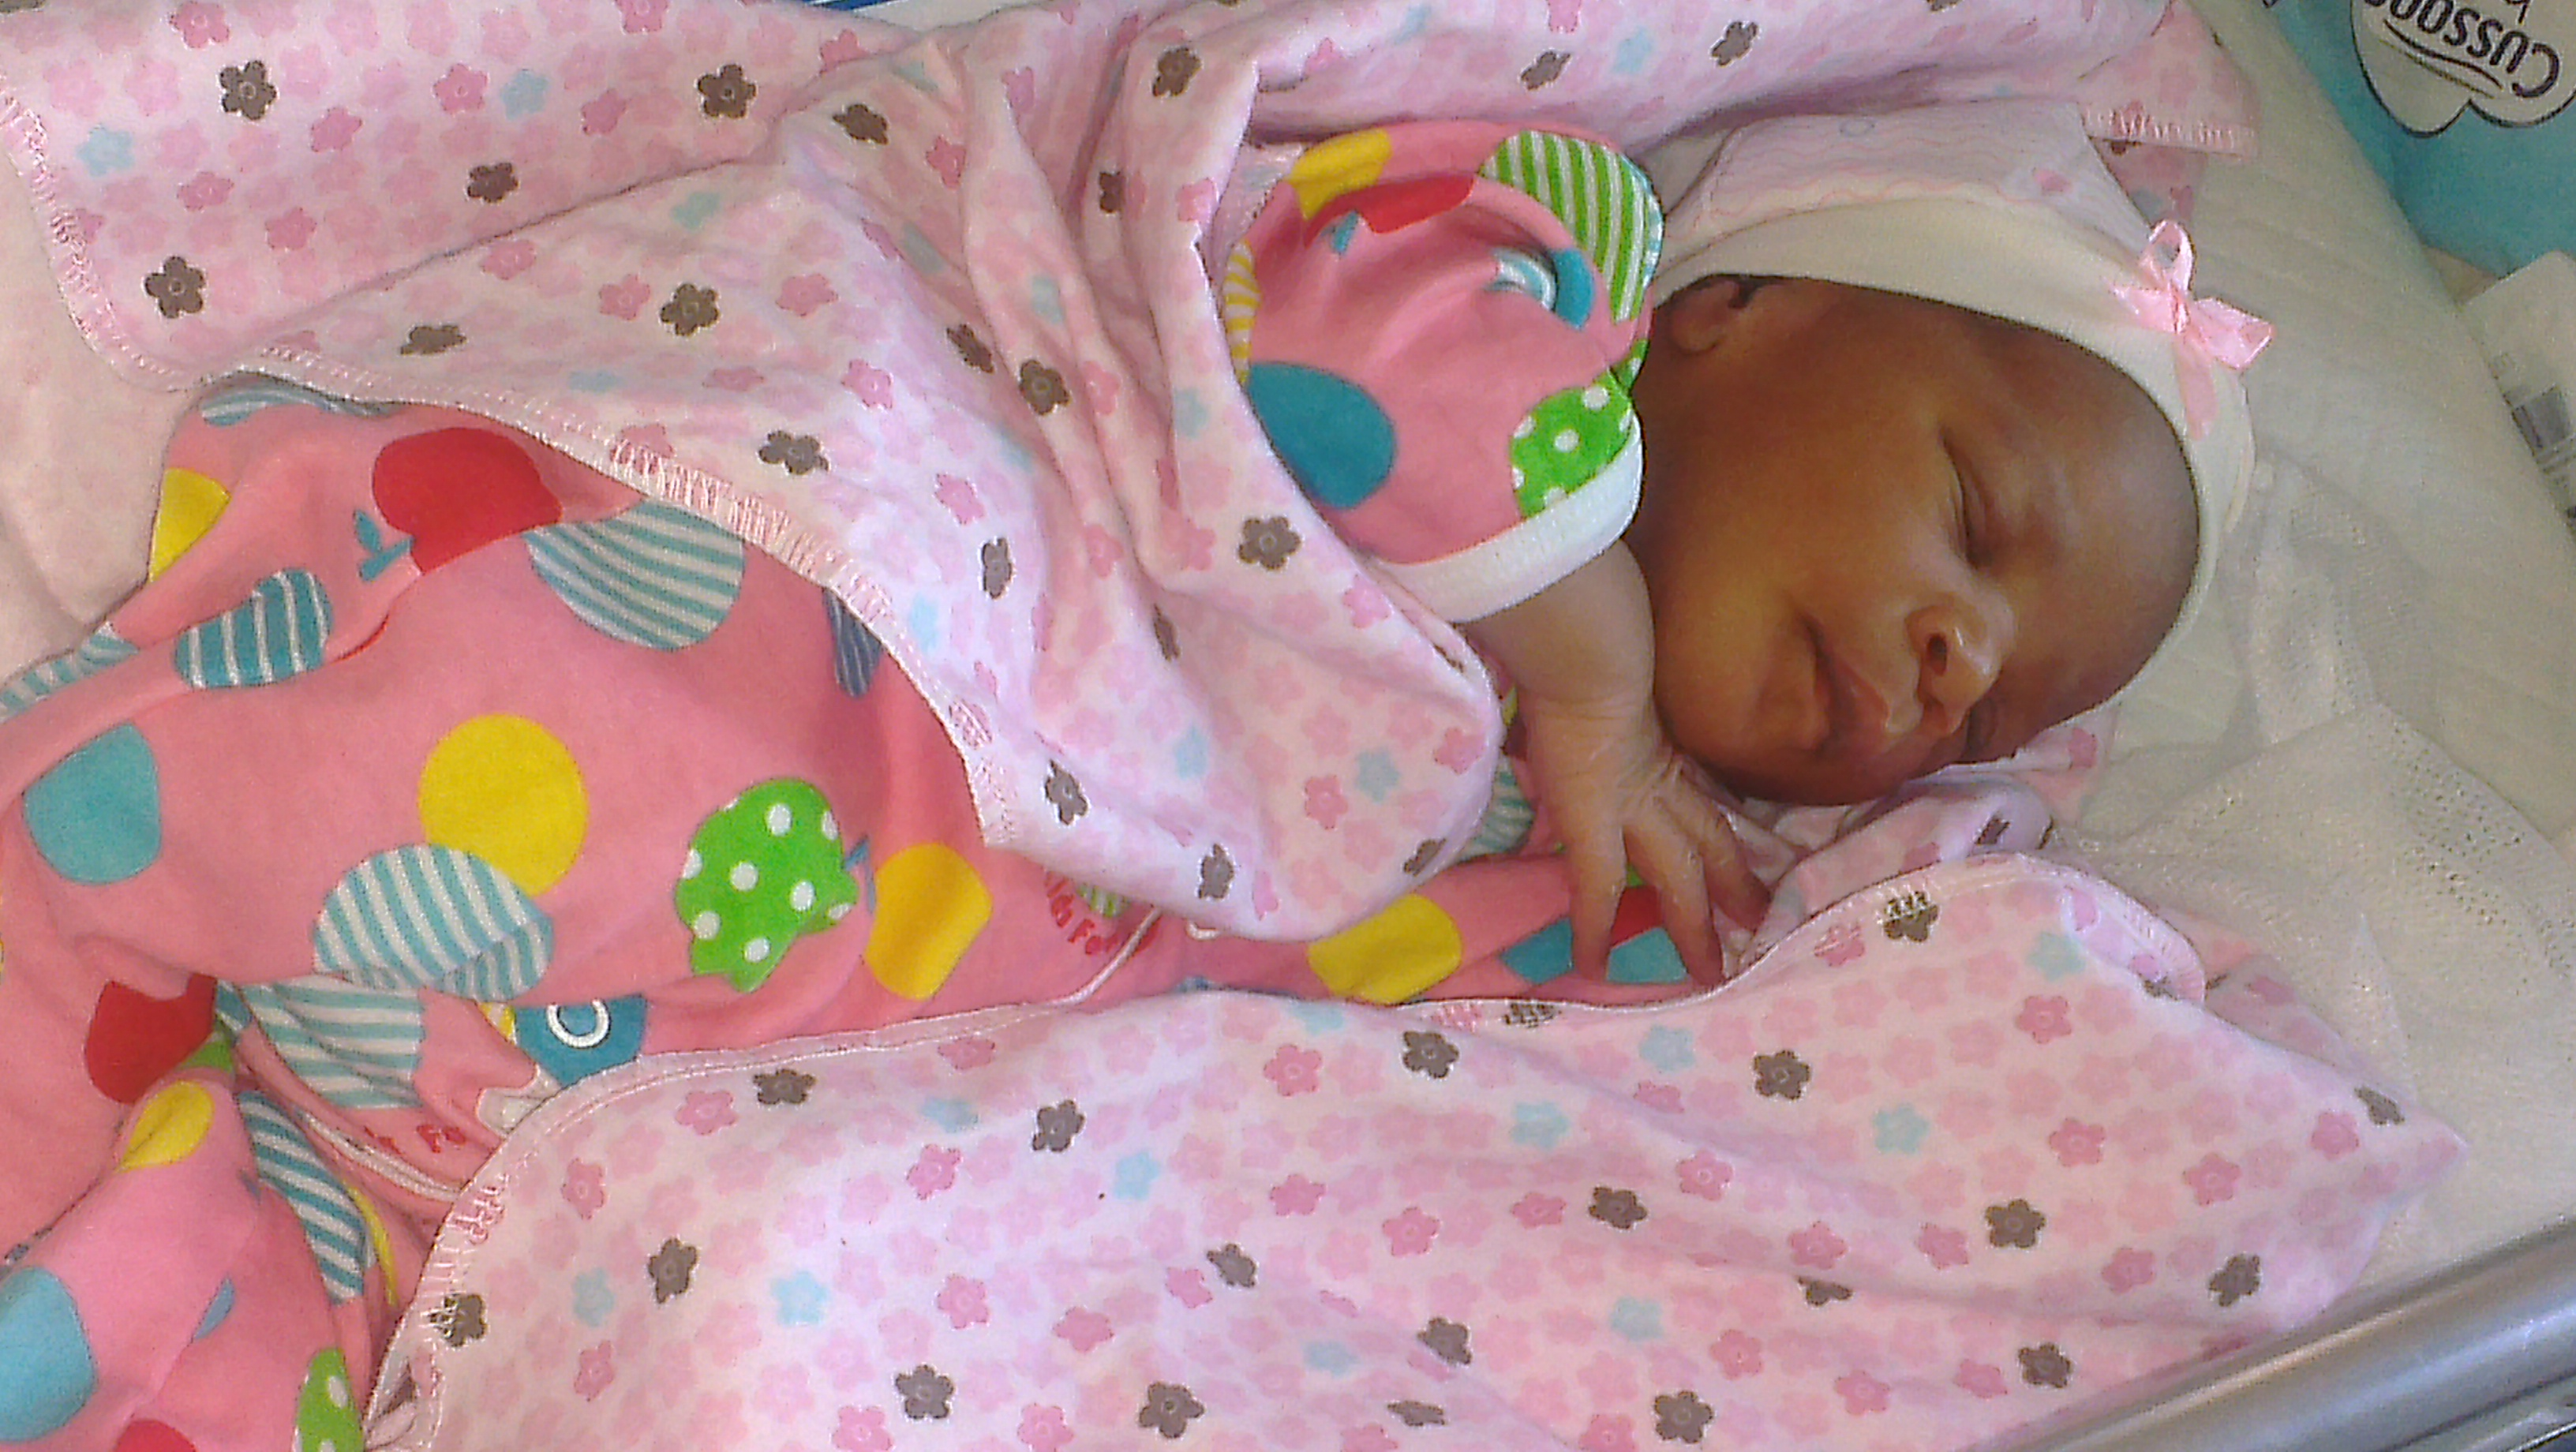
\includegraphics[width=1.03\linewidth]{Images/baby4.jpg}
	%\caption[R GUI]{}
	%\caption{$\mathrm{\huge{R}}$ GUI}
	%\label{fig:RPage}
\end{figure}
\end{frame}

\begin{frame}[t]{Our baby's name}
\begin{itemize}
	\item Our baby's names are:
	\begin{enumerate}
		\item \textbf{\textcolor{blue!45!black}{Obaloluwa}}
	\item
	\textbf{\textcolor{blue!45!black}{Samuel}} 
	\pause
	\item
	\textbf{\textcolor{blue!45!black}{Oluwapelumi}} 
	\pause
%	\item
%	\textbf{\textcolor{blue!45!black}{Oluwapelumi}} 
%	\pause
		\item
		 \textbf{\textcolor{blue!45!black}{Morireoluwa}} 
		\pause
		\item \textbf{\textcolor{blue!45!black}{Akinfolarin}} 
		\pause
		\item \textcolor{blue!45!black}{Ayomikun} 
		\pause
		\item \textcolor{blue!45!black}{Eniibukun} 
		\pause
	%	\item \textcolor{blue!45!black}{Oluwapelumi} 
	%	\pause
		\item \textcolor{blue!45!black}{Oluwanifemi}
		\pause
		\item \textcolor{blue!45!black}{Oluwadamilola} 
		\pause
	%	\item \textcolor{blue!45!black}{Samuel}
		
	\end{enumerate}
\end{itemize}

\end{frame}




\begin{frame}[t]{Our baby's name}
\begin{itemize}
	\item Others are:
	\begin{enumerate}
		\item \textcolor{blue!45!black}{Abimifunoluwa}
		\pause
		\item \textcolor{blue!45!black}{Oluwasegun}
		\pause
		\item \textcolor{blue!45!black}{Olawolemi}
		\pause
		\item \textcolor{blue!45!black}{Oluwakorede}
		\item \textcolor{blue!45!black}{Titioluwalope}
		\pause
		\item \textcolor{blue!45!black}{Jesusemilore}
		\pause
		\item \textcolor{blue!45!black}{Temitayo}
		\pause
		\item \textcolor{blue!45!black}{Olasubomi}
	\end{enumerate}
\end{itemize}

\end{frame}










\begin{frame}{Appreciation}
\textcolor{blue!45!black}{\Large{Thank you for coming}}
\begin{figure}[t]
	\centering
	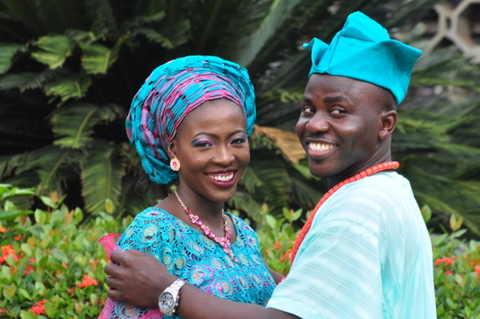
\includegraphics[width=0.80\linewidth]{Images/ThankU1.JPG}
	%\caption[R GUI]{}
	%\caption{$\mathrm{\huge{R}}$ GUI}
	%\label{fig:RPage}
\end{figure}
\end{frame}

\end{document}